% !TeX root = ../quantum.tex

\chapter{رمزنگاری پسا‌کوانتومی}
\label{chap:12}


	این فصل به مفاهیم رمزنگاری پسا‌کوانتومی\LTRfootnote{Post-quantum cryptography (PQC)} اختصاص دارد. پس از مقدمه، موضوعات زیر در حوزه رمزنگاری مبتنی بر مشبکه\LTRfootnote{Lattice-based cryptography} تشریح می‌شوند: رمزنگاری مبتنی بر یادگیری با خطا\LTRfootnote{Learning with errors (LWE)} ماتی\LTRfootnote{Module LWE}، رمزنگاری مبتنی بر \lr{LWE} حلقوی\LTRfootnote{Ring LWE}، امضاهای دیجیتال\LTRfootnote{Digital signatures} مبتنی بر مشبکه و توابع هش\LTRfootnote{Hash functions} مبتنی بر مشبکه. در ادامه، مفاهیم رمزنگاری مبتنی بر کد\LTRfootnote{Code-based cryptography} شامل طرح رمزگذاری مک‌الیس\LTRfootnote{McEliece encryption scheme}، سیستم رمزنگاری نیدرایتر\LTRfootnote{Niederreiter cryptosystem} و رمزگذاری مبتنی بر کدگذاری بررسی توازن کم‌چگال (\lr{LDPC}) شبه‌دوری\LTRfootnote{Quasi-cyclic (QC)-LDPC} شرح داده می‌شوند. در بخش بعدی، مفاهیم ترکیبی\LTRfootnote{Hybrid} \lr{QKD-PQC} معرفی می‌گردند که در آن‌ها \lr{QKD} و \lr{PQC} به‌صورت تعاملی عمل می‌کنند. در این طرح، ارسال کلید خام از طریق زیرسیستم \lr{QKD} انجام می‌شود، در حالی که مصالحه اطلاعات\LTRfootnote{Information reconciliation} از طریق زیرسیستم \lr{PQC} صورت می‌گیرد. موضوعات زیر در این بخش تشریح می‌شوند: رمزگذاری ترکیبی \lr{PQC-QKD}، زیرسیستم رمزگذاری مک‌الیس مبتنی بر کدگذاری \lr{LDPC} جفت‌شده فضایی\LTRfootnote{Spatially coupled LDPC} و رمزگذاری ترکیبی \lr{QKD-PQC} میدان-دوقلو\LTRfootnote{Twin field (TF)-QKD}. سپس تمرکز به سمت رمزنگاری مبتنی بر هش\LTRfootnote{Hash-based cryptography} معطوف می‌شود. پس از معرفی مفاهیم پایه رمزنگاری مبتنی بر هش، شامل طرح امضای یک‌بار مصرف لمپورت\LTRfootnote{Lamport’s one-time signature}، دو طرح مرتبط تشریح می‌شوند: طرح امضای یک‌بار مصرف وینترنیتز\LTRfootnote{Winternitz one-time signature (W-OTS)} (\lr{W-OTS}) و طرح امضای مرکل\LTRfootnote{Merkle signature scheme (MMS)} (\lr{MMS}) که برای امضاهای چندبار مصرف کاربرد دارد. پس از آن، مفاهیم مرتبط با رمزنگاری چندمتغیره\LTRfootnote{Multivariate cryptography} تشریح می‌شوند.


\section{مقدمه}
\label{sec:12-1}
توزیع کلید کوانتومی (\lr{QKD})، که در فصل‌های قبل تشریح شد، از فیزیک بنیادی برای تضمین امنیت بهره می‌برد \cite{12-1, 12-2, 12-3, 12-4, 12-5, 12-6}؛ برخلاف فرضیات ریاضی اثبات‌نشده‌ای که برای امنیت محاسباتی\LTRfootnote{Computational security} استفاده می‌شوند. اگرچه اولین نمایش \lr{QKD} ماهواره به زمین \cite{12-5} به تحقیقات مخابرات کوانتومی\LTRfootnote{Quantum communications (QuCom)} شتاب بخشیده است، اما همچنان چندین مانع برای کاربردهای گسترده وجود دارد. به‌عنوان مثال، تلفات کانال هم نرخ کلید مخفی (\lr{SKR})\LTRfootnote{Secret-key rate (SKR)} در هر مُد واحد و هم مسافت دستیابی‌پذیر را در یک مصالحه نرخ-تلفات\LTRfootnote{Rate-loss tradeoff} محدود می‌کند. برای غلبه بر این موانع، اخیراً دو رویکرد زیر محبوب شده‌اند: (الف) توسعه رله‌های کوانتومی\LTRfootnote{Quantum relays} \cite{12-7} و (ب) معرفی مفهوم رله‌های مورد اعتماد\LTRfootnote{Trusted relays} \cite{12-8}. با این حال، رله‌های کوانتومی نیازمند حافظه‌های کوانتومی با طول زمان زیاد و درهم‌تنیدگی\LTRfootnote{Entanglement} با وفاداری بالا هستند که در حال حاضر به‌صورت تجاری در دسترس نیستند. از سوی دیگر، در کاربردهای عملی، تأیید اعتماد برای رله بین هر دو گره در یک شبکه نوری دشوار است. \lr{QKD} در واقع می‌تواند برای ساخت شبکه‌های امن آینده استفاده شود. متأسفانه، نرخ‌های \lr{SKR} برای سیستم‌های \lr{QKD} متغیر گسسته\LTRfootnote{Discrete variable (DV)} (\lr{DV}) فعلی بسیار پایین است، به‌طوری که «مخزن»\LTRfootnote{Pool} کلید کوانتومی متناظر که کلیدهای مخفی و امن را ذخیره می‌کند، اغلب خالی می‌ماند و بدین ترتیب عملکرد این شبکه‌ها را مختل می‌کند. سیستم‌های \lr{QKD} متغیر پیوسته\LTRfootnote{Continuous variable (CV)} (\lr{CV}) با مشکل زمان مرده\LTRfootnote{Dead time} مواجه نیستند و می‌توانند برای بهبود نرخ‌های \lr{SKR} استفاده شوند، اما همان‌طور که در مرجع \cite{12-6} نشان داده شده است، مسافت دستیابی‌پذیر در طرح‌های \lr{CV-QKD} در مقایسه با طرح‌های \lr{DV-QKD} میدان-دوقلو (\lr{TF}) به‌طور قابل‌توجهی کوتاه‌تر است \cite{12-9, 12-10, 12-11}. به‌عنوان یک نمونه، نویسندگان در مرجع \cite{12-12} از فیبر چند‌هسته‌ای\LTRfootnote{Multicore fiber} با $37$ هسته برای دستیابی به نرخ \lr{SKR} برابر با $105.7$ مگابیت بر ثانیه استفاده کردند، اما مسافت ارسال تنها $7.9$ کیلومتر بود.







رمزنگاری پسا‌کوانتومی\LTRfootnote{Post-quantum cryptography (PQC)} (\lr{PQC}) یک جایگزین توصیه‌شده برای \lr{QKD} است \cite{12-13, 12-14, 12-15, 12-16, 12-17, 12-18, 12-19}. ایده کلیدی در پس \lr{PQC}، طراحی و پیاده‌سازی پروتکل‌های کلید عمومی است که توسط هیچ کامپیوتر کوانتومی قابل شکستن نباشند. الگوریتم‌های غالب \lr{PQC} را می‌توان در چهار دسته قرار داد: (الف) رمزنگاری مبتنی بر مشبکه\LTRfootnote{Lattice-based cryptography} که در بخش \ref{sec:12-2} تشریح خواهد شد، (ب) رمزنگاری مبتنی بر کد\LTRfootnote{Code-based cryptography} که در بخش \ref{sec:12-3} توصیف می‌گردد، (ج) رمزنگاری مبتنی بر هش\LTRfootnote{Hash-based cryptography} در بخش \ref{sec:12-4} و (د) رمزنگاری چندمتغیره\LTRfootnote{Multivariate cryptography} در بخش \ref{sec:12-5}.

با این حال، مشابه امنیت محاسباتی، هیچ مدرکی وجود ندارد که ثابت کند الگوریتم‌های \lr{PQC} توسط الگوریتم‌های کوانتومی پیچیده نفوذناپذیر هستند. به‌عنوان یک مثال توصیفی، الگوریتم‌های رمزنگاری مشبکه بر این حدس استوار هستند که هیچ الگوریتم زمان چند‌جمله‌ای وجود ندارد که مسائل مشبکه را با فاکتورهای چند‌جمله‌ای تقریب بزند \cite{12-17}. علاوه‌ بر این، اغلب رمزنگاری مشبکه بر پایه توابع هش مقاوم در برابر برخورد\LTRfootnote{Collision resistance hash functions} بنا شده است؛ مانند $\bm{u} = \bm{A}\bm{x}$ که در آن $\bm{x}$ بردار خصوصی آلیس، $\bm{u}$ بردار عمومی آلیس و $\bm{A}$ ماتریس عمومی $m \times n$ توصیف‌کننده مشبکه است که ستون‌های آن بردارهای پایه مشبکه هستند. ایو برای تعیین بردار خصوصی آلیس از طریق $\bm{x} = \bm{A}^{-1}\bm{u}$ و در نتیجه شکستن پروتکل \lr{PQC}، نیاز به اجرای یک الگوریتم معکوس‌سازی ماتریس کوانتومی کارآمد، مشابه الگوریتم هرو-حسیدیم-لوید\LTRfootnote{Harrow-Hassidim-Lloyd (HHL) algorithm} (\lr{HHL}) دارد \cite{12-20}. الگوریتم \lr{HHL} یک شتاب‌دهی نمایی نسبت به الگوریتم‌های کلاسیک ارائه می‌دهد. برای غلبه بر مشکلات اصلی هر دو پروتکل \lr{QKD} و \lr{PQC}، یک گزینه استفاده از پروتکل‌های مشترک \lr{QKD-PQC} است \cite{12-21}؛ با این حال، حتی اگر مسافت ارسال پروتکل \lr{PM-TF-QKD} تطبیق فاز \cite{12-10} بتواند دوبرابر شود، نرخ کلید مخفی همچنان چندین مرتبه بزرگی کمتر از نرخ داده‌های مورد استفاده در سیستم‌های مخابرات نوری پیشرفته است. ما در مقاله اخیر خود \cite{12-1}، استفاده از یک استراتژی جدید را برای غلبه بر مشکلات فوق در \lr{QKD} و \lr{PQC} به‌صورت هم‌زمان پیشنهاد داده‌ایم. با توجه به پایین بودن نرخ کلید خام در پروتکل‌های \lr{QKD}، برای دستیابی به دنباله امن مشترک، پیشنهاد می‌کنیم که از طرح‌های سنتی \lr{QKD} تنها در مرحله مقداردهی اولیه\LTRfootnote{Initialization stage} پروتکل‌های پیشنهادی استفاده شود. برخلاف طرح‌های متداول \lr{QKD}، دنباله امن مشترک ما یک کلید متقارت نخواهد بود، بلکه سیستم‌های رمزنگاری پیشنهادی را مقداردهی اولیه می‌کند. ایده کلیدی این است که از دنباله امن مشترکِ حاصل از \lr{QKD} نه به‌عنوان یک کلید امن، بلکه برای موارد زیر استفاده شود: (الف) یک دنباله امن از کلیدهای عمومی؛ (ب) دانه‌ها\LTRfootnote{Seeds} برای مولدهای «تابع هش» تصادفی متناظر توسط آلیس و باب؛ (ج) پارامترهایی برای مقداردهی اولیه پروتکل‌ها؛ و غیره. این دنباله‌های امن بسیار کوتاه‌تر از طول کلید برای رمزگذاری پد یک‌بار مصرف خواهند بود، بنابراین نرخ \lr{SKR} در پروتکل \lr{QKD} مربوطه، یک نگرانی عمده نخواهد بود. طرح‌های ترکیبی \lr{QKD-PQC} در بخش \ref{sec:12-6} تشریح خواهند شد.






\section{رمزنگاری مبتنی بر مشبکه}
\label{sec:12-2}
مشبکه\LTRfootnote{Lattice} توسط $n$ بردار مستقل خطی\LTRfootnote{Linearly independent vectors} $\bm{b}_1, \dots, \bm{b}_n \in \mathbb{R}^m$ تولید می‌شود، که در آن $\mathbb{R}$ مجموعه اعداد حقیقی است، و به‌صورت زیر تعریف می‌گردد:
\begin{equation}
	L(\bm{b}_1, \cdots, \bm{b}_n) = \{x_i \bm{b}_i \mid x_i \in \mathbb{Z}\}, \quad m \geq n
	\label{eq:12-1}
\end{equation}

که در آن $\mathbb{Z}$ نشان‌دهنده مجموعه اعداد صحیح است. با نوشتن بردارهای پایه $m$-مؤلفه‌ای به‌صورت ستونی، ماتریس $m \times n$ به‌صورت 
$\bm{A} = [\bm{b}_1 \,\, \bm{b}_2 \ \dots \ \bm{b}_n] \in \mathbb{R}^{m \times n}$ به‌دست می‌آید، به‌طوری که می‌توانیم مشبکه را به‌صورت $L(\bm{b}_1, \dots, \bm{b}_n) = L(\bm{A}) = \{ \bm{A}\bm{x} \mid \bm{x} \in \mathbb{Z}^m \}$ بازتعریف کنیم.

با داشتن یک مشبکه، مسائل خاصی وجود دارند که حل آن‌ها دشوار است، از جمله:
\begin{itemize}
	\item \textbf{مسئله کوتاه‌ترین بردار\LTRfootnote{Shortest vector problem (SVP)} (\lr{SVP}):} با داشتن مشبکه‌ای که توسط پایه $\bm{A}$ توصیف شده است، کوتاه‌ترین بردار غیرصفر در مشبکه $L(\bm{A})$ را تعیین کنید؛ نمونه‌ای از آن در شکل \ref{fig:12-1} ارائه شده است.
	\item \textbf{مسئله نزدیک‌ترین بردار\LTRfootnote{Closest vector problem (CVP)} (\lr{CVP}):} با داشتن مشبکه‌ای که توسط پایه $\bm{A}$ توصیف شده و یک بردار هدف $\bm{t}$ که در مشبکه نیست، بردار $\bm{v}$ در مشبکه را که نزدیک‌ترین بردار به بردار هدف $\bm{t}$ است، تعیین کنید.
	\item \textbf{رمزگشایی با فاصله محدود\LTRfootnote{Bounded distance decoding}:} مشابه با \lr{CVP}، نقطه مشبکه‌ی $\bm{s}$ را که نزدیک‌ترین نقطه به بردار دریافتی (هدف) $\bm{r}$ ($\bm{t}$) است، تعیین کنید.
\end{itemize}

مسئلهٔ مرتبط دیگر، مسئلهٔ کوتاه‌ترین بردارهای مستقل\LTRfootnote{Shortest Independent Vectors Problem (SIVP)} (\lr{SIVP}) است که می‌توان آن را به‌صورت زیر بیان کرد: با فرض شبکه‌ای\LTRfootnote{Lattice} با پایهٔ\LTRfootnote{Basis} $\bm{A} \in \mathbb{Z}^{m \times n}$، $n$ بردار مستقل خطی $\bm{S} = [\bm{s}_1 \quad \bm{s}_2 \quad \cdots \quad \bm{s}_n]$ را به‌گونه‌ای تعیین کنید که $\|\bm{S}\| = \mathrm{max}_i \|\bm{s}_i\|$ کمینه شود، که در آن $\|\bm{s}_i\|$ نُرم\LTRfootnote{Norm} بردار $\bm{s}_i$ است. یکی از پرکاربردترین نُرم‌ها، نُرم اقلیدسی\LTRfootnote{Euclidean Norm} است که به‌صورت زیر تعریف می‌شود:
$
	\|\bm{s}_i\| = \left(\sum_j s_{ij}^2\right)^{1/2}
	\label{eq:12-2}
$.


\begin{figure}[ht]
	\centering
	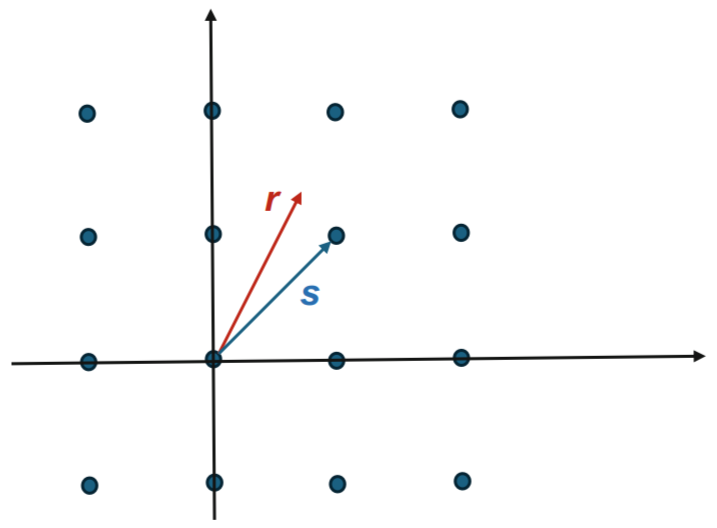
\includegraphics[width=0.8\textwidth]{chapters/figs/fig-12-1}
	\caption{تصویرسازی مسئله کوتاه‌ترین بردار.}
	\label{fig:12-1}
\end{figure}

\subsection{رمزنگاری مبتنی بر یادگیری با خطای ماتی (LWE)}
\label{subsec:12-2-1}
الگوریتم‌های رمزنگاری مبتنی بر مشبکه با برخی از مسائل فهرست‌شده در بالا مرتبط هستند. در رمزنگاری مبتنی بر یادگیری با خطا\LTRfootnote{Learning with errors (LWE)} (\lr{LWE})، ما عناصر بردارهای پایه را به‌صورت تصادفی از $\mathbb{Z}_q^n$ انتخاب می‌کنیم، که در آن $\mathbb{Z}_q$ مجموعه اعداد صحیح در پیمانه $q$ است.






ماتریس $\bm{A}$ و پارامتر $q$ به‌صورت عمومی در دسترس قرار می‌گیرند. یک پروتکل ساده مبتنی بر \lr{LWE}، معروف به یادگیری با خطای ماتی\LTRfootnote{Module learning with errors (module-LWE)} (\lr{module-LWE})، می‌تواند به‌صورت زیر توصیف شود. بردار خصوصی (محرمانه)\LTRfootnote{Private (secret) vector} آلیس، $|s_A\rangle$، از طریق $|p_A\rangle = \bm{A}|s_A\rangle$ با بردار عمومی\LTRfootnote{Public vector} $|p_A\rangle$ در ارتباط است. تولید ماتریس $\bm{A}$ و بردار عمومی آلیس $|p_A\rangle$ نشان‌دهنده گام تولید کلید است. باب بردار خصوصی $\langle s_B|$ و بردار خطا\LTRfootnote{Error vector} $\langle e|$ را تولید کرده و از آن‌ها برای تولید بردار خام عمومی $\langle p_B|$ و اسکالر\LTRfootnote{Scalar} $c$، که بخشی از رمزنگاشت\LTRfootnote{Ciphertext} است، به‌صورت زیر استفاده می‌کند: $\langle p_B| = \langle s_B|\bm{A} + \langle e|$ و $c = \langle s_B|p_A\rangle + e + bq/2$، که در آن $b \in \{0,1\}$ بیتی است که باید رمزگذاری شود. مؤلفه‌های خطا $e_i$ ($i = 1, \dots, m$) و $e$ به‌صورت تصادفی انتخاب می‌شوند اما باید بسیار کوچک‌تر از $q/4$ باشند. بنابراین، باب گام رمزگذاری را برای به‌دست آوردن رمزنگاشتِ متشکل از $\langle p_B|$ و $c$ انجام می‌دهد. آلیس با به‌کارگیری بردار خصوصی خود $|s_A\rangle$ عمل رمزگشایی را به‌صورت زیر انجام می‌دهد:
\begin{equation}
	\begin{aligned}
		b' &= \frac{2}{q} (c - \langle p_B|s_A\rangle) = \frac{2}{q} \left[ \underbrace{\langle s_B|\bm{A}|s_A\rangle}_{|p_A\rangle} + e + bq/2 - (\langle s_B|\bm{A} + \langle e|) |s_A\rangle \right] \\
		&= \frac{2}{q} [\langle s_B|\bm{A}|s_A\rangle + e + bq/2 - \langle s_B|\bm{A}|s_A\rangle - \langle e|s_A\rangle] \\
		&= b + \frac{2}{q} (e - \langle e|s_A\rangle).
	\end{aligned}
	\label{eq:12-2}
\end{equation}
با توجه به اینکه مقدار $\frac{2}{q}(e - \langle e|s_A\rangle)$ عدد کوچکی است و مانند نویز عمل می‌کند، بیت رمزگشایی‌شده $b'$ با بیت باب یعنی $b$ برابر خواهد بود.

همچنین می‌توان تفسیر زیر را ارائه داد \cite{12-22}. در گام تولید کلید، آلیس فهرست-$\bm{A}$ را به‌صورت برداری با طول $n$ از اعداد تصادفی در پیمانه $q$ تولید می‌کند که اعضای آن $A_i \in \mathbb{Z}_q$ هستند. او همچنین یک الگوی خطا به طول $n$ با مؤلفه‌هایی تولید می‌کند که آن‌ها نیز از $\mathbb{Z}_q$ اما کوچک‌تر از $q/n$ هستند. او سپس فهرست-$\bm{B}$ را به‌صورت زیر ایجاد می‌کند:
\begin{equation}
	B_i = A_i s + e_i \pmod q,
	\label{eq:12-3}
\end{equation}
که در آن $s$ عدد محرمانه است. او فهرست‌های $\bm{A}$ و $\bm{B}$ را به‌عنوان کلید عمومی منتشر می‌کند. باب با نمونه‌برداری و انتخاب $K$ نمونه از فهرست-$\bm{B}$، بیت $b$ را به‌صورت زیر رمزگذاری می‌کند:
\begin{equation}
	v = \sum_{j \in \text{Positions}} B_j - bq/2 \mod q,
	\label{eq:12-4}
\end{equation}

که در آن مجموعه \textit{مکان‌ها}\LTRfootnote{Positions} نشان‌دهنده محل نمونه‌ها است. برای رمزگشایی، آلیس ابتدا عدد $u$ را از طریق رابطه زیر ایجاد می‌کند:
\begin{equation}
	u = \sum_{j \in \text{Positions}} A_j \mod q,
	\label{eq:12-3}
\end{equation}

و بیت باب را با استفاده از رابطه زیر و از طریق گرد کردن\LTRfootnote{Rounding} رمزگشایی می‌کند:
\begin{equation}
	b' = \frac{2}{q}\left(v - su \mod q\right),
	\label{eq:12-5}
\end{equation}














